%!mode::"Tex:UTF-8"
\PassOptionsToPackage{unicode}{hyperref}
\PassOptionsToPackage{naturalnames}{hyperref}
\documentclass[hyperref,cs4size,titlepage]{ctexart}
%\documentclass{article}
%\usepackage{luatexja-fontspec}
%\setmainjfont{SimSun}
%\usepackage{fullpage}
\usepackage{geometry}
\usepackage{parskip}
\usepackage{physics}
\usepackage{amsmath}
\usepackage{amssymb}
\usepackage{xcolor}
%\usepackage[colorlinks,urlcolor=red,citecolor=green,anchorcolor=blue]{hyperref}
\usepackage{array}
\usepackage{longtable}
\usepackage{multirow}
\usepackage{comment}
\usepackage{graphicx}
\usepackage{cite}
\usepackage{slashbox}
\usepackage{titlesec}
%\usepackage{intent}
\usepackage{fancyhdr}
\usepackage{float}
\geometry{left=3cm,right=2.5cm,top=3cm,bottom=2.5cm}
\pagestyle{fancy}
\fancyhead[L]{}
\fancyhead[LO]{\zihao{-5}薛定谔方程的重整化和有效理论}
\fancyhead[RO]{\zihao{-5}\leftmark}
%\fancyhead[R]{}
%\fancyfoot[LE]{-\thepage-}
\fancyfoot[RO]{-\thepage-}
\fancyfoot[C]{}
\renewcommand{\headrule}{%
\hrule width\headwidth height1.2pt \vspace{1pt}%
\hrule width\headwidth}
\hypersetup{colorlinks,linkcolor=blue,citecolor=blue,CJKbookmarks=true}
\CTEXsetup[format+={\zihao{4}\songti}]{section}
\CTEXsetup[format+={\zihao{4}\songti}]{subsection}
\CTEXsetup[format+={\zihao{4}\songti}]{subsubsection}
\makeatletter % `@' now normal "letter"
\@addtoreset{equation}{section}
\makeatother  % `@' is restored as "non-letter"
\renewcommand\theequation{\oldstylenums{\thesection}%
                   .\oldstylenums{\arabic{equation}}}
\titleformat{\paragraph}[block]{\normalsize\bfseries}{\theparagraph}{1em}{}
\title{\zihao{3}薛定谔方程的重整化和有效理论}
\author{\zihao{-4}黄应生}
\date{}
\begin{document}
\maketitle
\pagestyle{empty}
\clearpage
\pagenumbering{roman}
\songti\tableofcontents
\clearpage
\pagestyle{fancy}
\section*{摘要}
\markboth{摘要}{}
\clearpage
\section*{Abstract}
\markboth{Abstract}{}
\clearpage
\pagenumbering{arabic}
\begin{figure}
  \centering
  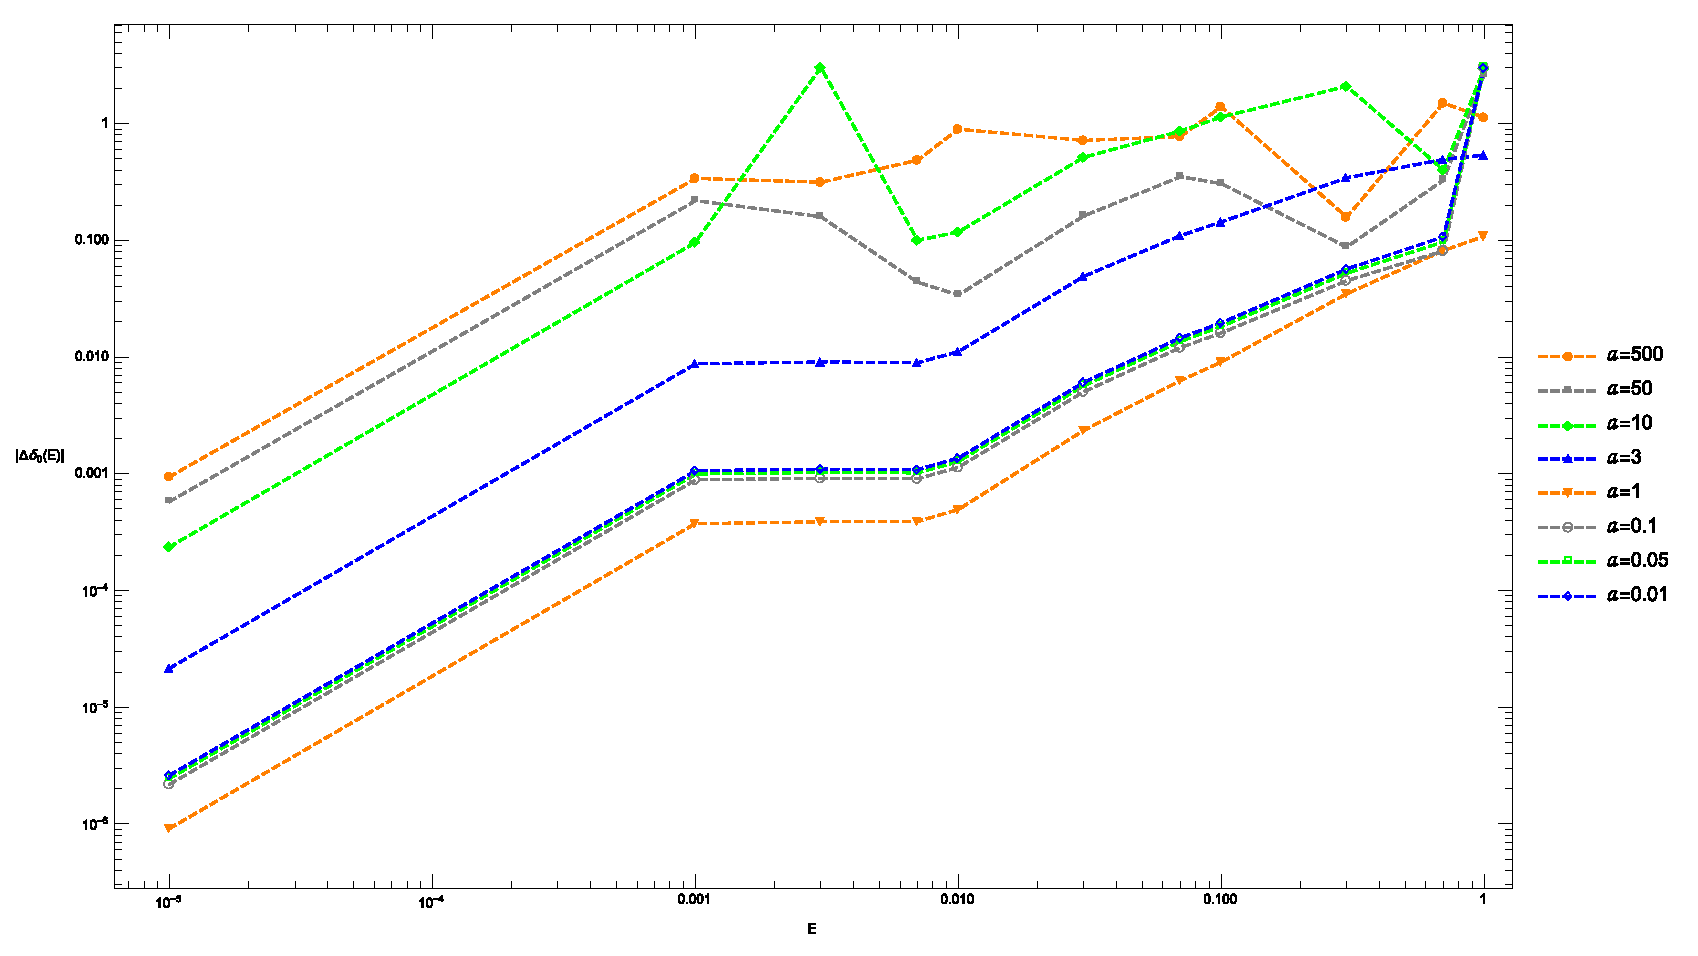
\includegraphics[width=6in]{Test_PhaseShift_Various_a.eps}
  \caption{$\alpha=1$,$m=1$}
\end{figure}
\begin{figure}
  \centering
  \includegraphics[width=6in]{{Test_Determine_a_Alpha=0.1&m=0.1}.eps}
  \caption{$\alpha=0.1$,$m=0.1$}
\end{figure}
\clearpage
\begin{figure}
  \centering
  \includegraphics[width=6in]{{Test_Determine_a_Alpha=1&m=0.1}.eps}
  \caption{$\alpha=1$,$m=0.1$}
\end{figure}
\begin{figure}
  \centering
  \includegraphics[width=6in]{{Test_Determine_a_Alpha=0.01&m=0.1}.eps}
  \caption{$\alpha=0.01$,$m=0.1$}
\end{figure}
\begin{figure}
  \centering
  \includegraphics[width=6in]{{Test_Determine_a_Alpha=0.1&m=0.01}.eps}
  \caption{$\alpha=0.1$,$m=0.01$}
\end{figure}
\begin{figure}
  \centering
  \includegraphics[width=6in]{{Test_Determine_a_Alpha=0.1&m=1}.eps}
  \caption{$\alpha=0.1$,$m=1$}
\end{figure}
\begin{figure}
  \centering
  \includegraphics[width=6in]{{Test_Determine_a_Alpha=0.01&m=0.01}.eps}
  \caption{$\alpha=0.01$,$m=0.01$}
\end{figure}
\clearpage
\begin{figure}[!htbp]
\begin{minipage}[t]{0.5\linewidth}
  \centering
  \includegraphics[width=1\textwidth]{{Test_Determine_a_Alpha=0.01&m=10}.eps}
\end{minipage}
\begin{minipage}[t]{0.5\linewidth}
  \centering
  \includegraphics[width=1\textwidth]{{Test_Determine_a_Alpha=0.1&m=1}.eps}
\end{minipage}\\

\begin{minipage}[t]{0.5\linewidth}
  \centering
  \includegraphics[width=1\textwidth]{{Test_Determine_a_Alpha=0.1&m=10}.eps}
\end{minipage}
\begin{minipage}[t]{0.5\linewidth}
  \centering
  \includegraphics[width=1\textwidth]{{Test_Determine_a_Alpha=0.01&m=100}.eps}
\end{minipage}\\

\begin{minipage}[t]{0.5\linewidth}
  \centering
  \includegraphics[width=1\textwidth]{{Test_Determine_a_Alpha=1&m=10}.eps}
\end{minipage}
\begin{minipage}[t]{0.5\linewidth}
  \centering
  \includegraphics[width=1\textwidth]{{Test_Determine_a_Alpha=0.1&m=100}.eps}
\end{minipage}
\caption{Determine a}
\end{figure}
\begin{figure}[!htbp]
\begin{minipage}[t]{0.5\linewidth}
  \centering
  \includegraphics[width=1\textwidth]{{Test_Determine_Coulomb_a_Alpha=0.01&m=10}.eps}
\end{minipage}
\begin{minipage}[t]{0.5\linewidth}
  \centering
  \includegraphics[width=1\textwidth]{{Test_Determine_Coulomb_a_Alpha=0.1&m=1}.eps}
\end{minipage}\\

\begin{minipage}[t]{0.5\linewidth}
  \centering
  \includegraphics[width=1\textwidth]{{Test_Determine_Coulomb_a_Alpha=0.1&m=10}.eps}
\end{minipage}
\begin{minipage}[t]{0.5\linewidth}
  \centering
  \includegraphics[width=1\textwidth]{{Test_Determine_Coulomb_a_Alpha=0.01&m=100}.eps}
\end{minipage}\\

\begin{minipage}[t]{0.5\linewidth}
  \centering
  \includegraphics[width=1\textwidth]{{Test_Determine_Coulomb_a_Alpha=1&m=10}.eps}
\end{minipage}
\begin{minipage}[t]{0.5\linewidth}
  \centering
  \includegraphics[width=1\textwidth]{{Test_Determine_Coulomb_a_Alpha=0.1&m=100}.eps}
\end{minipage}
\caption{Determine a}
\end{figure}
\begin{figure}[!tp]
\begin{minipage}[t]{0.329\linewidth}
  \centering
  \includegraphics[width=1\textwidth]{{Plot_c1_veus_a_Alpha=0.1&m=1}.eps}
\end{minipage}
\begin{minipage}[t]{0.329\linewidth}
  \centering
  \includegraphics[width=1\textwidth]{{Plot_c1_veus_a_Alpha=0.3&m=1}.eps}
\end{minipage}
\begin{minipage}[t]{0.329\linewidth}
  \centering
  \includegraphics[width=1\textwidth]{{Plot_c1_veus_a_Alpha=0.4&m=1}.eps}
\end{minipage}
  \caption{有效势$V_{eff}^{(a^2)}$的耦合常数$c$对截断$a$的依赖}\label{cveusa}
\end{figure}
\subsection{$\psi(r)$}
$\psi_{eff}(r)$修正后表达式为:
\begin{equation}\label{psi0r}
  \psi_{true}(r)=\overline{\gamma}(r)\int\dd^3r\psi_{eff}\delta^3_a(\vb{r})+\overline{\eta}(r)a^2\int\dd^3r\psi_{eff}\laplacian{\delta^3_a(\vb{r})}+\mathcal{O}(a^3)
\end{equation}
这一关系仅在$r<a$时成立。
\begin{figure}[!htbp]
  \centering
  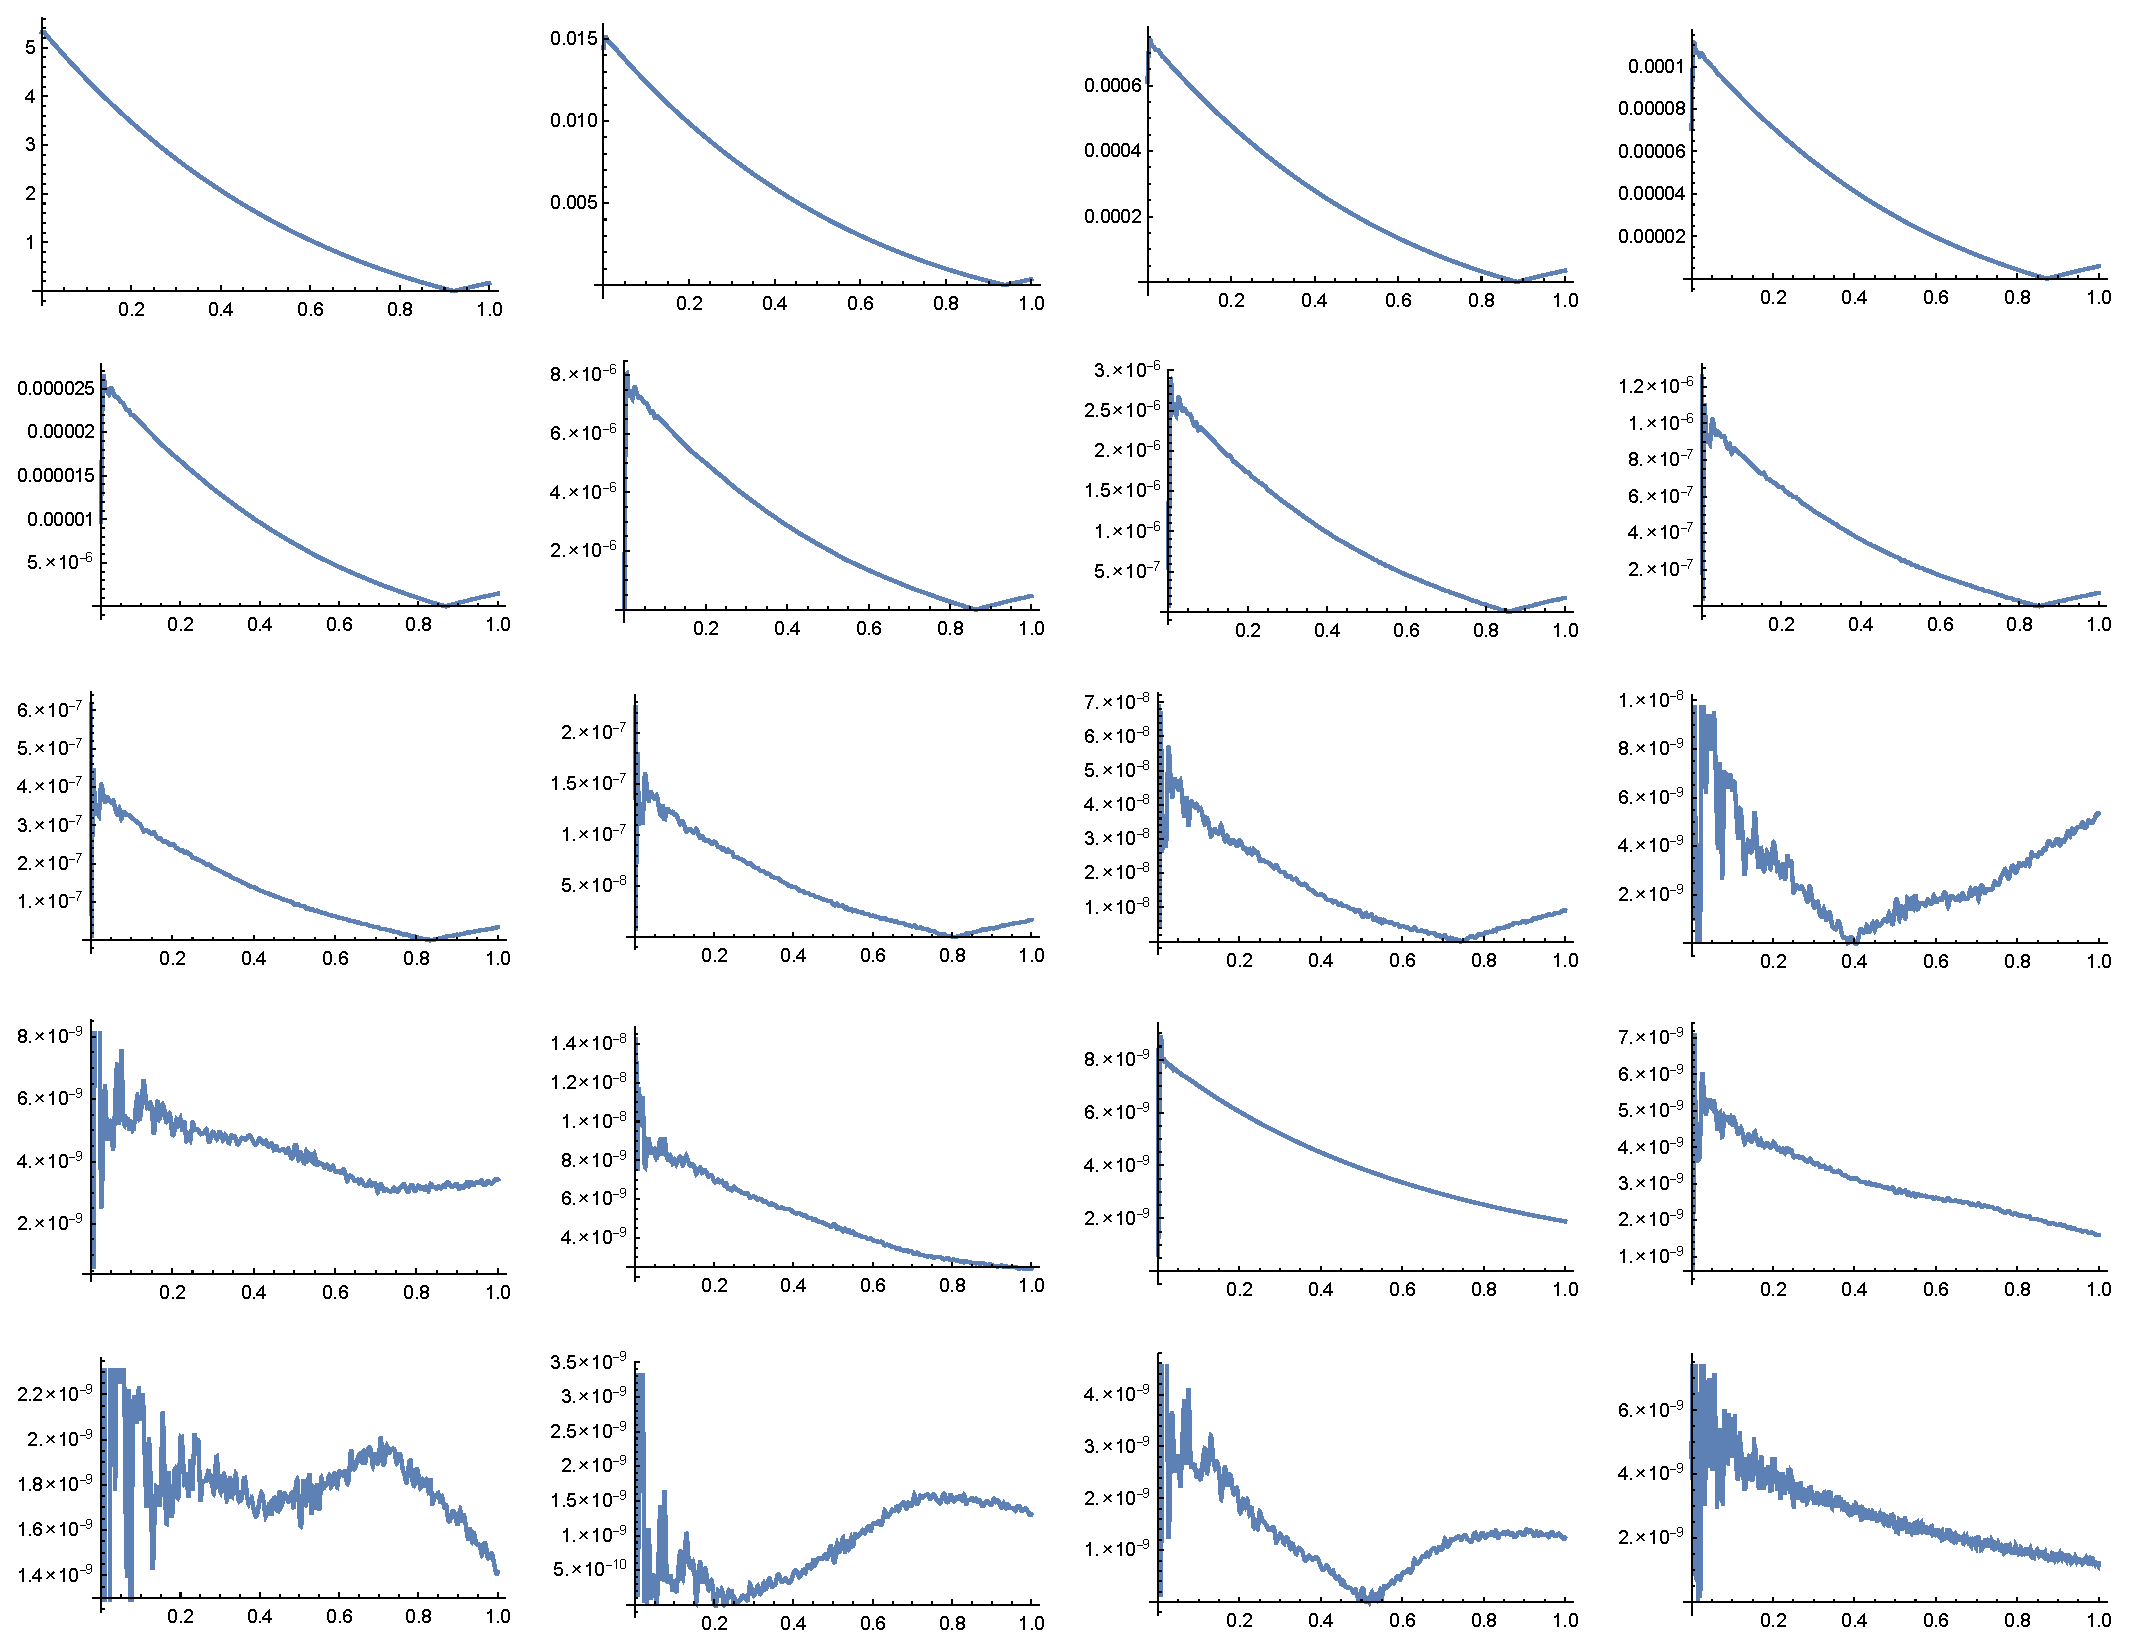
\includegraphics[width=6in]{psir.eps}
  \caption{$\psi_{eff}(r)$在前20个能级与真实波函数的对比}
\end{figure}\\
可以发现除了第一个能级之外,其它能级与真实波函数都符合得较好,并且能级越高,符合得越好。若$r>a$,则
\clearpage
\begin{figure}[!htbp]
  \centering
  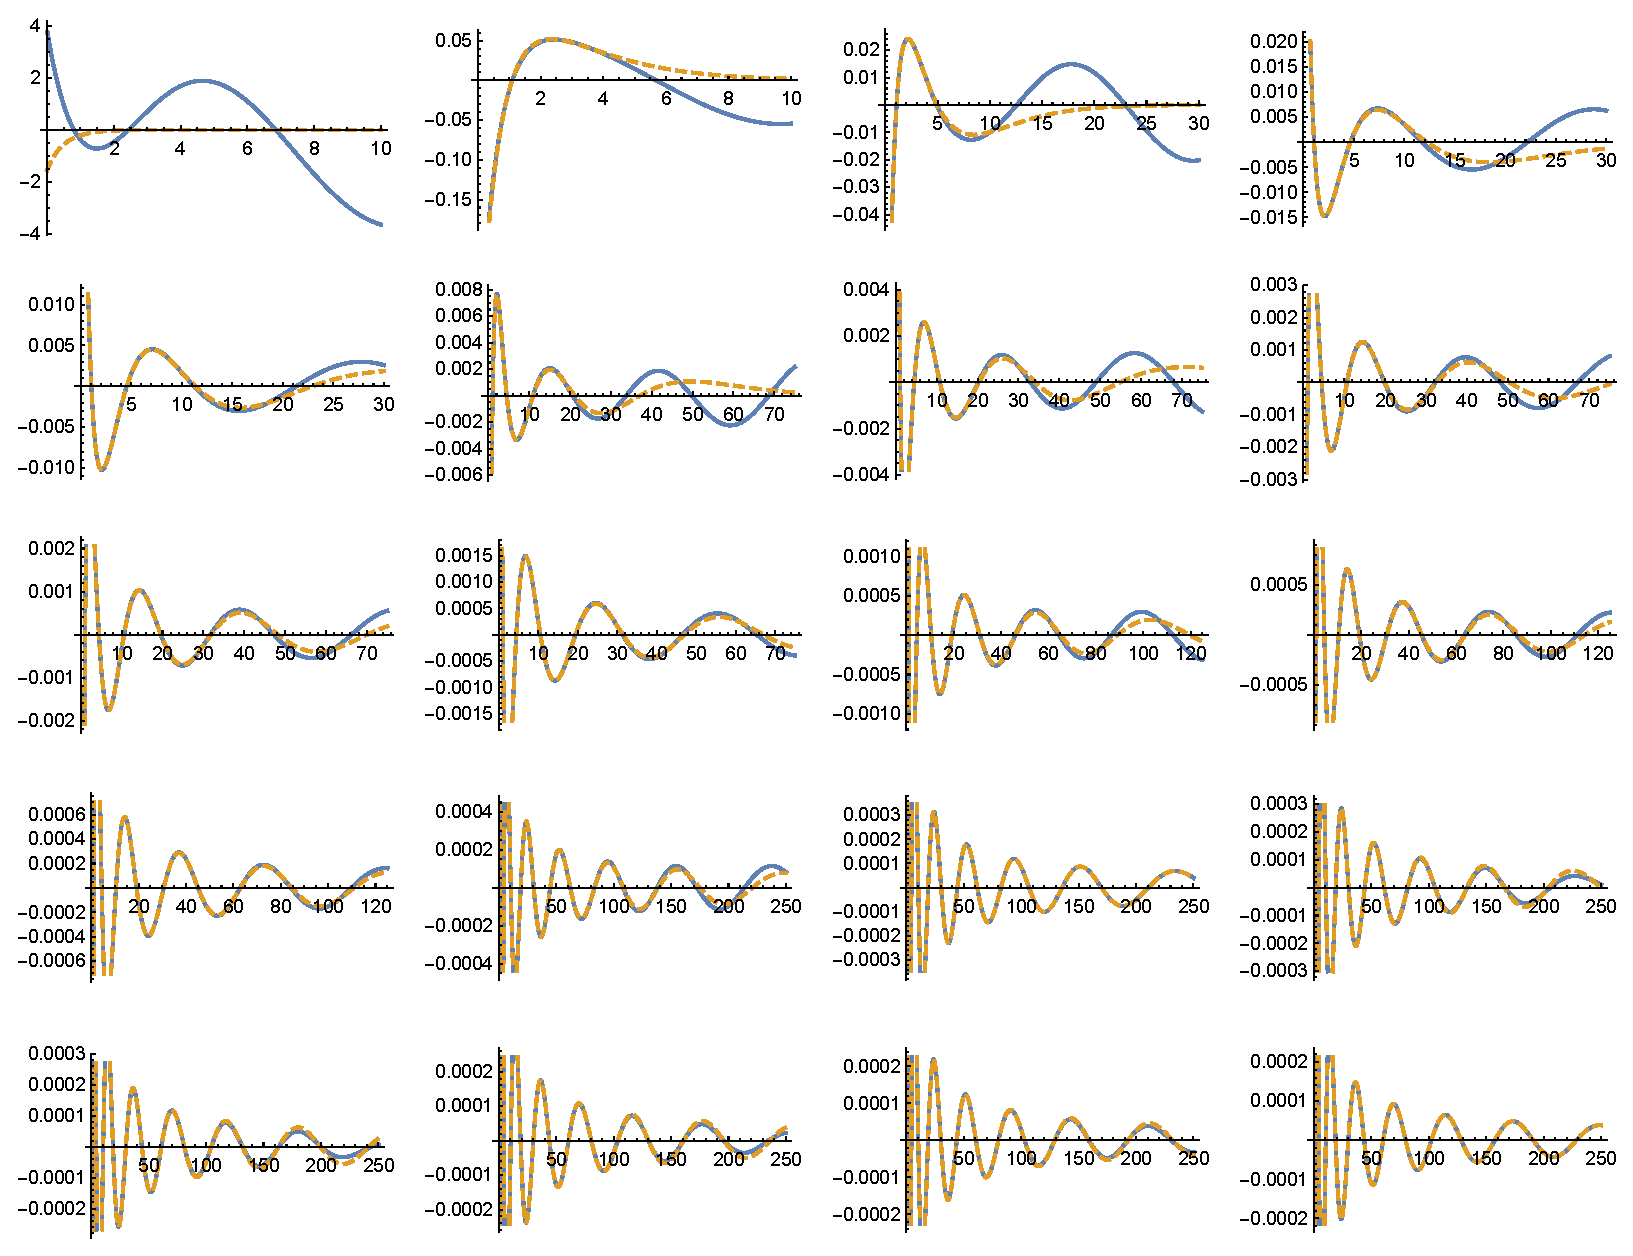
\includegraphics[width=6in]{psir_2.eps}
  \caption{$\psi_{eff}(r)(r>a)$在前20个能级与真实波函数的对比}
\end{figure}
但若再加上$\overline{Z}(r)\psi_{eff}(r)$,则可让$\psi_{true}(r)$在$r>a$时也能成立。

加上$\overline{Z}(r)$,$\psi_{true}(r)$可写为
\begin{equation}\label{psi0ra}
  \psi_{true}(r)=\overline{Z}(r)\psi_{eff}(r)+\overline{\gamma}(r)\int\dd^3r\psi_{eff}\delta^3_a(\vb{r})+\overline{\eta}(r)a^2\int\dd^3r\psi_{eff}\laplacian{\delta^3_a(\vb{r})}+\mathcal{O}(a^3)
\end{equation}
于是可以得到$\psi_{true}(r)$的图像。
\begin{figure}[!htbp]
  \centering
  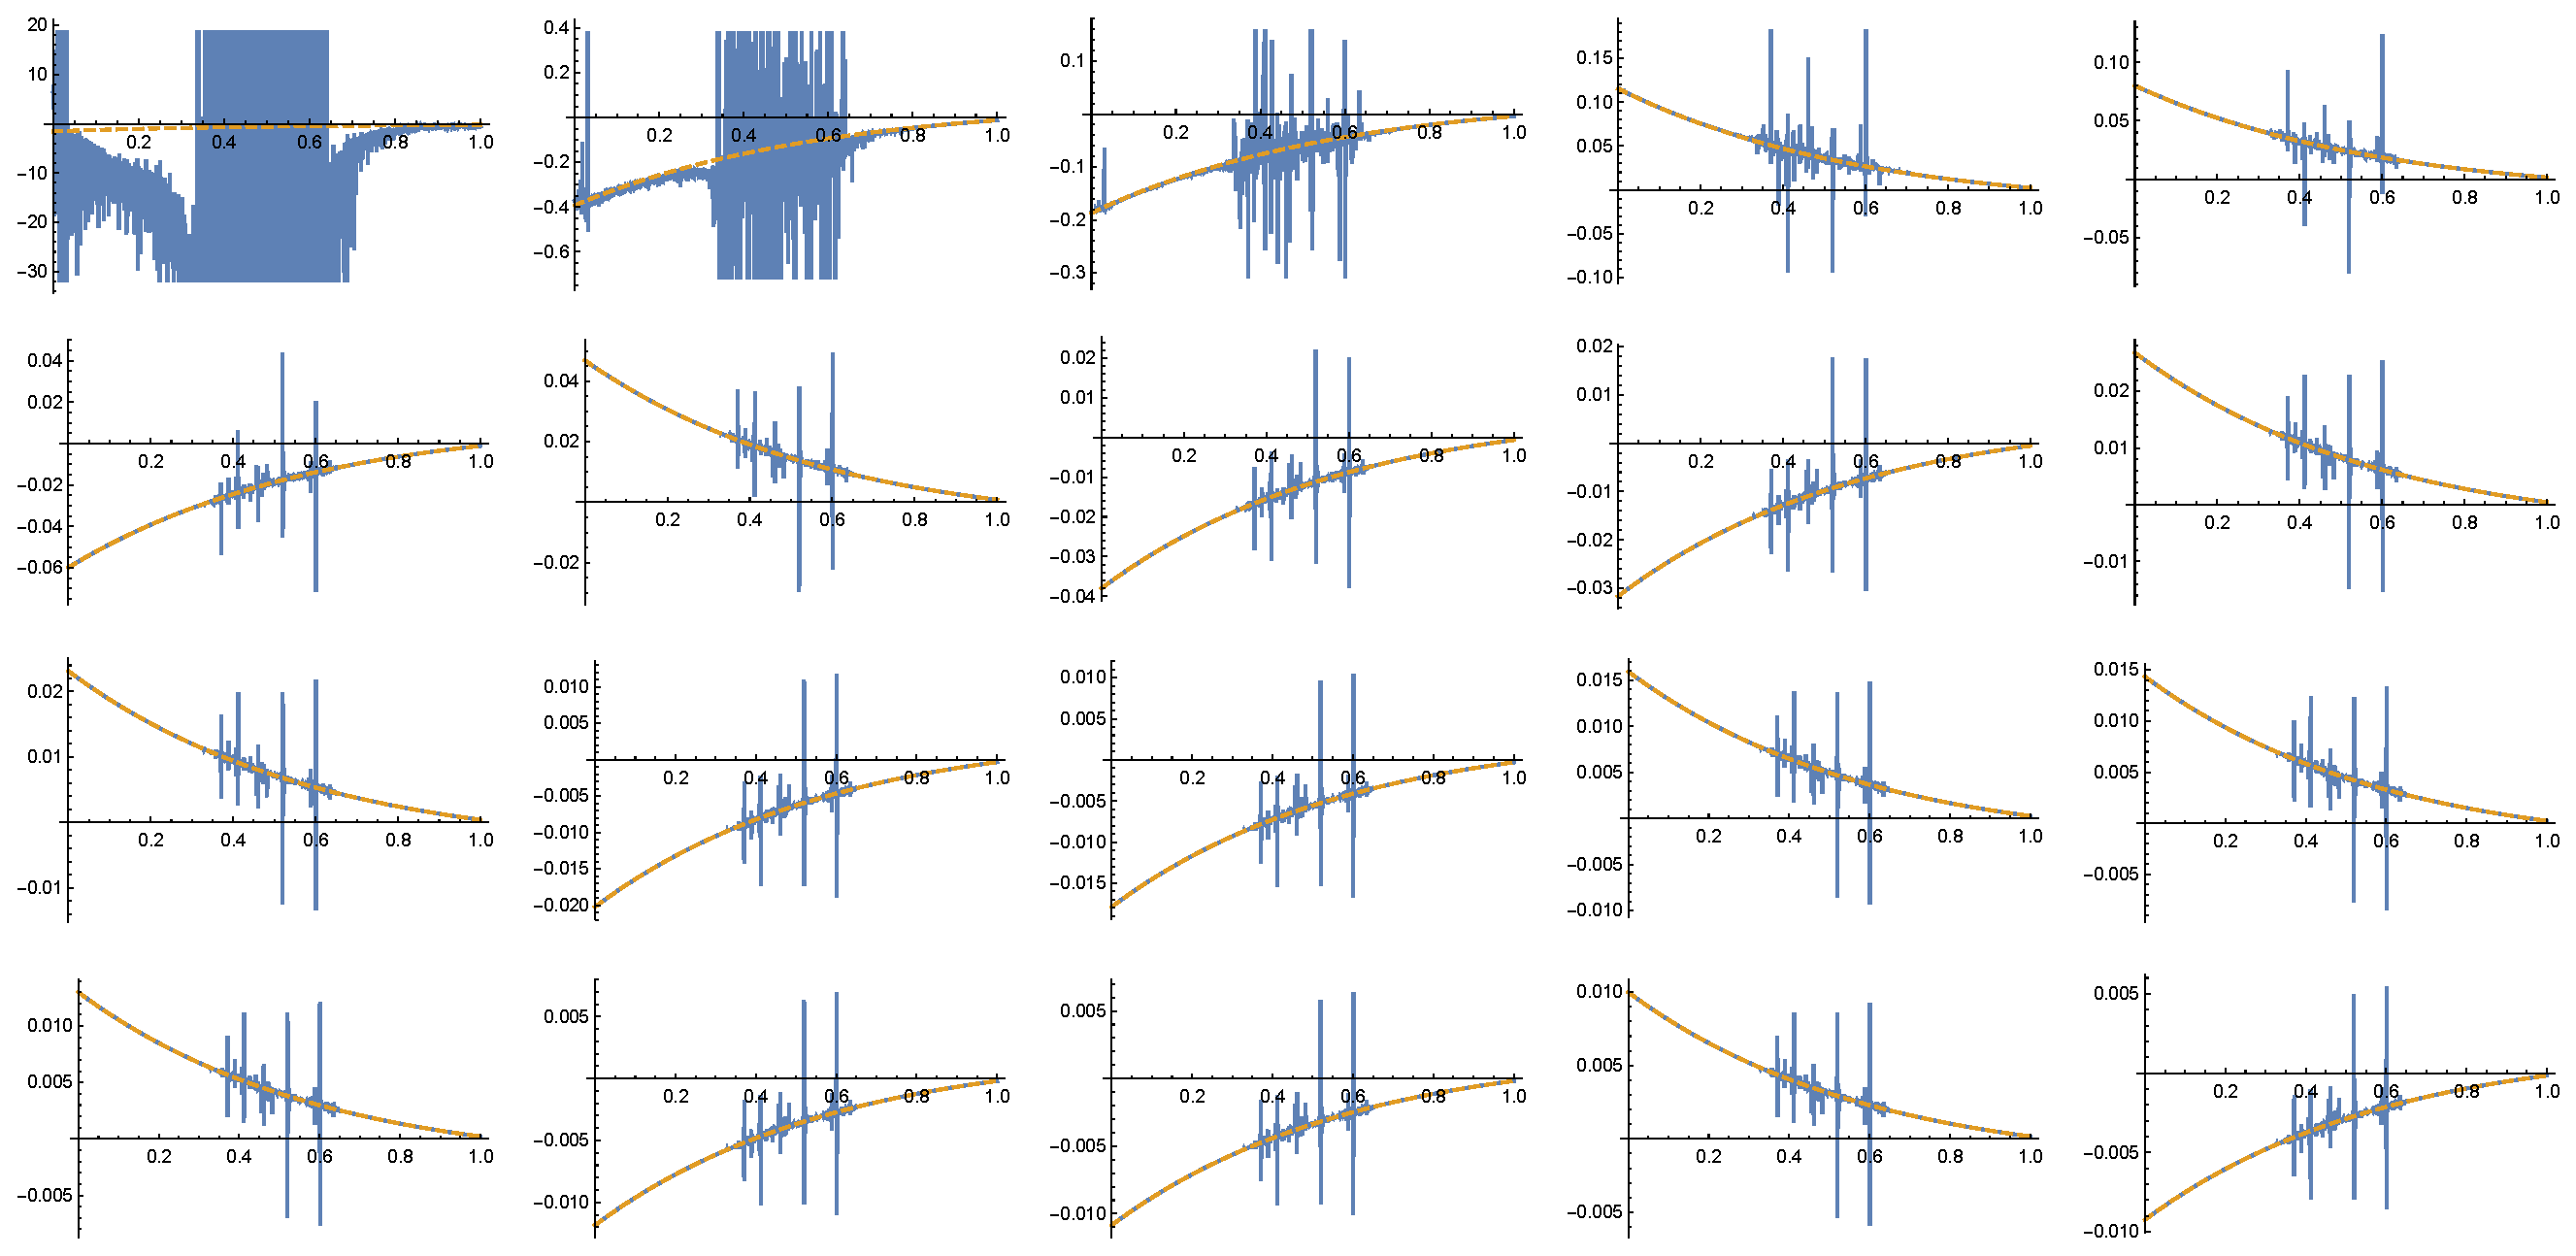
\includegraphics[width=6in]{psirmodified2.eps}
  \caption{$\psi_{eff}(r)(r>a)$在前20个能级与真实波函数的对比}
\end{figure}\\
可以发现,对于几乎所有能级(除了1S外),大范围的$r$内基本都与真实波函数一致。但是图像中的波函数并不是完全光滑的,这是因为\eqref{psi0ra}中的参数不止有一种可能,而不光滑的地方则是参数从一种可能跳到另一种可能所导致的。
\begin{figure}[!htbp]
  \centering
  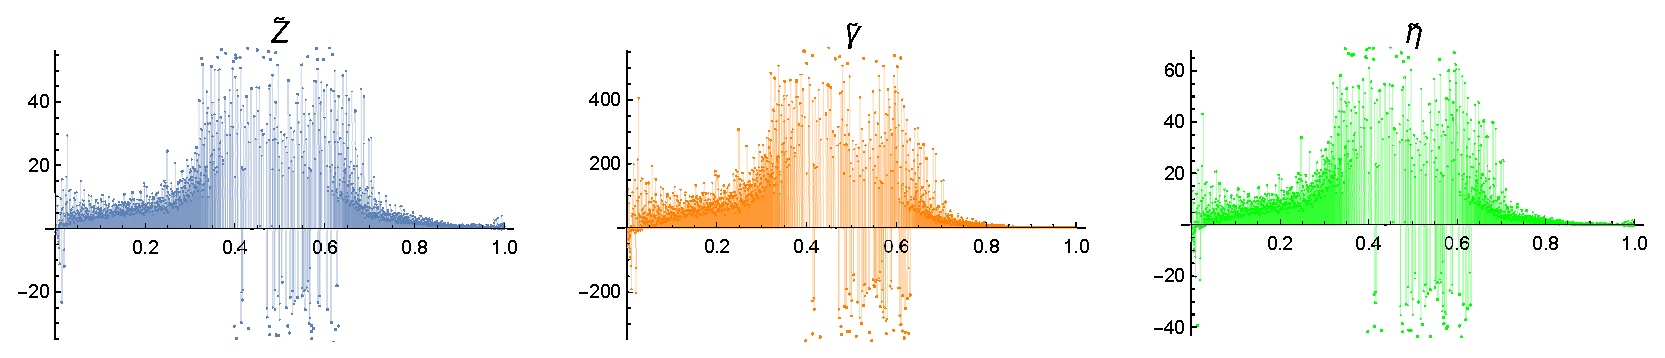
\includegraphics[width=6in]{psirmodified2_2.eps}
  \caption{$\overline{Z}(r)$、$\overline{\gamma}(r)$、$\overline{\eta}(r)$ 的取值}
\end{figure}

$\laplacian{\psi_{true}(r)}$同样可以用相同的办法求出。对方程\eqref{psi0r}左右同时求导后可以得到
\begin{alignat}{1}\label{psi0rl}
  \laplacian{\psi_{true}(r)}=&\overline{\gamma}(r)\int\dd^3r\psi_{eff}\delta^3_a(\vb{r})+\overline{\gamma'}(r)\int\dd^3r\laplacian{\bqty{\psi_{eff}\delta^3_a(\vb{r})}}+\overline{\eta}(r)a^2\int\dd^3r\psi_{eff}\laplacian{\delta^3_a(\vb{r})}
 \nonumber\\&+\overline{\eta'}(r)a^2\int\dd^3r\laplacian{\bqty{\psi_{eff}\laplacian{\delta^3_a(\vb{r})}}}+\mathcal{O}(a^3)
\end{alignat}
其中可以证明$\int\dd^3r\laplacian{\bqty{\psi_{eff}\delta^3_a(\vb{r})}}$与$\int\dd^3r\laplacian{\bqty{\psi_{eff}\laplacian{\delta^3_a(\vb{r})}}}$之值为0。于是\eqref{psi0rl}仅剩两项
\begin{equation}\label{psi0rl2}
  \laplacian{\psi_{true}(r)}=\overline{\gamma}(r)\int\dd^3r\psi_{eff}\delta^3_a(\vb{r})+\overline{\eta}(r)a^2\int\dd^3r\psi_{eff}\laplacian{\delta^3_a(\vb{r})}+\mathcal{O}(a^3)
\end{equation}
其形式与\eqref{psi0r}基本相同。画出$r<a$时的图像,则为
\begin{figure}[!htbp]
  \centering
  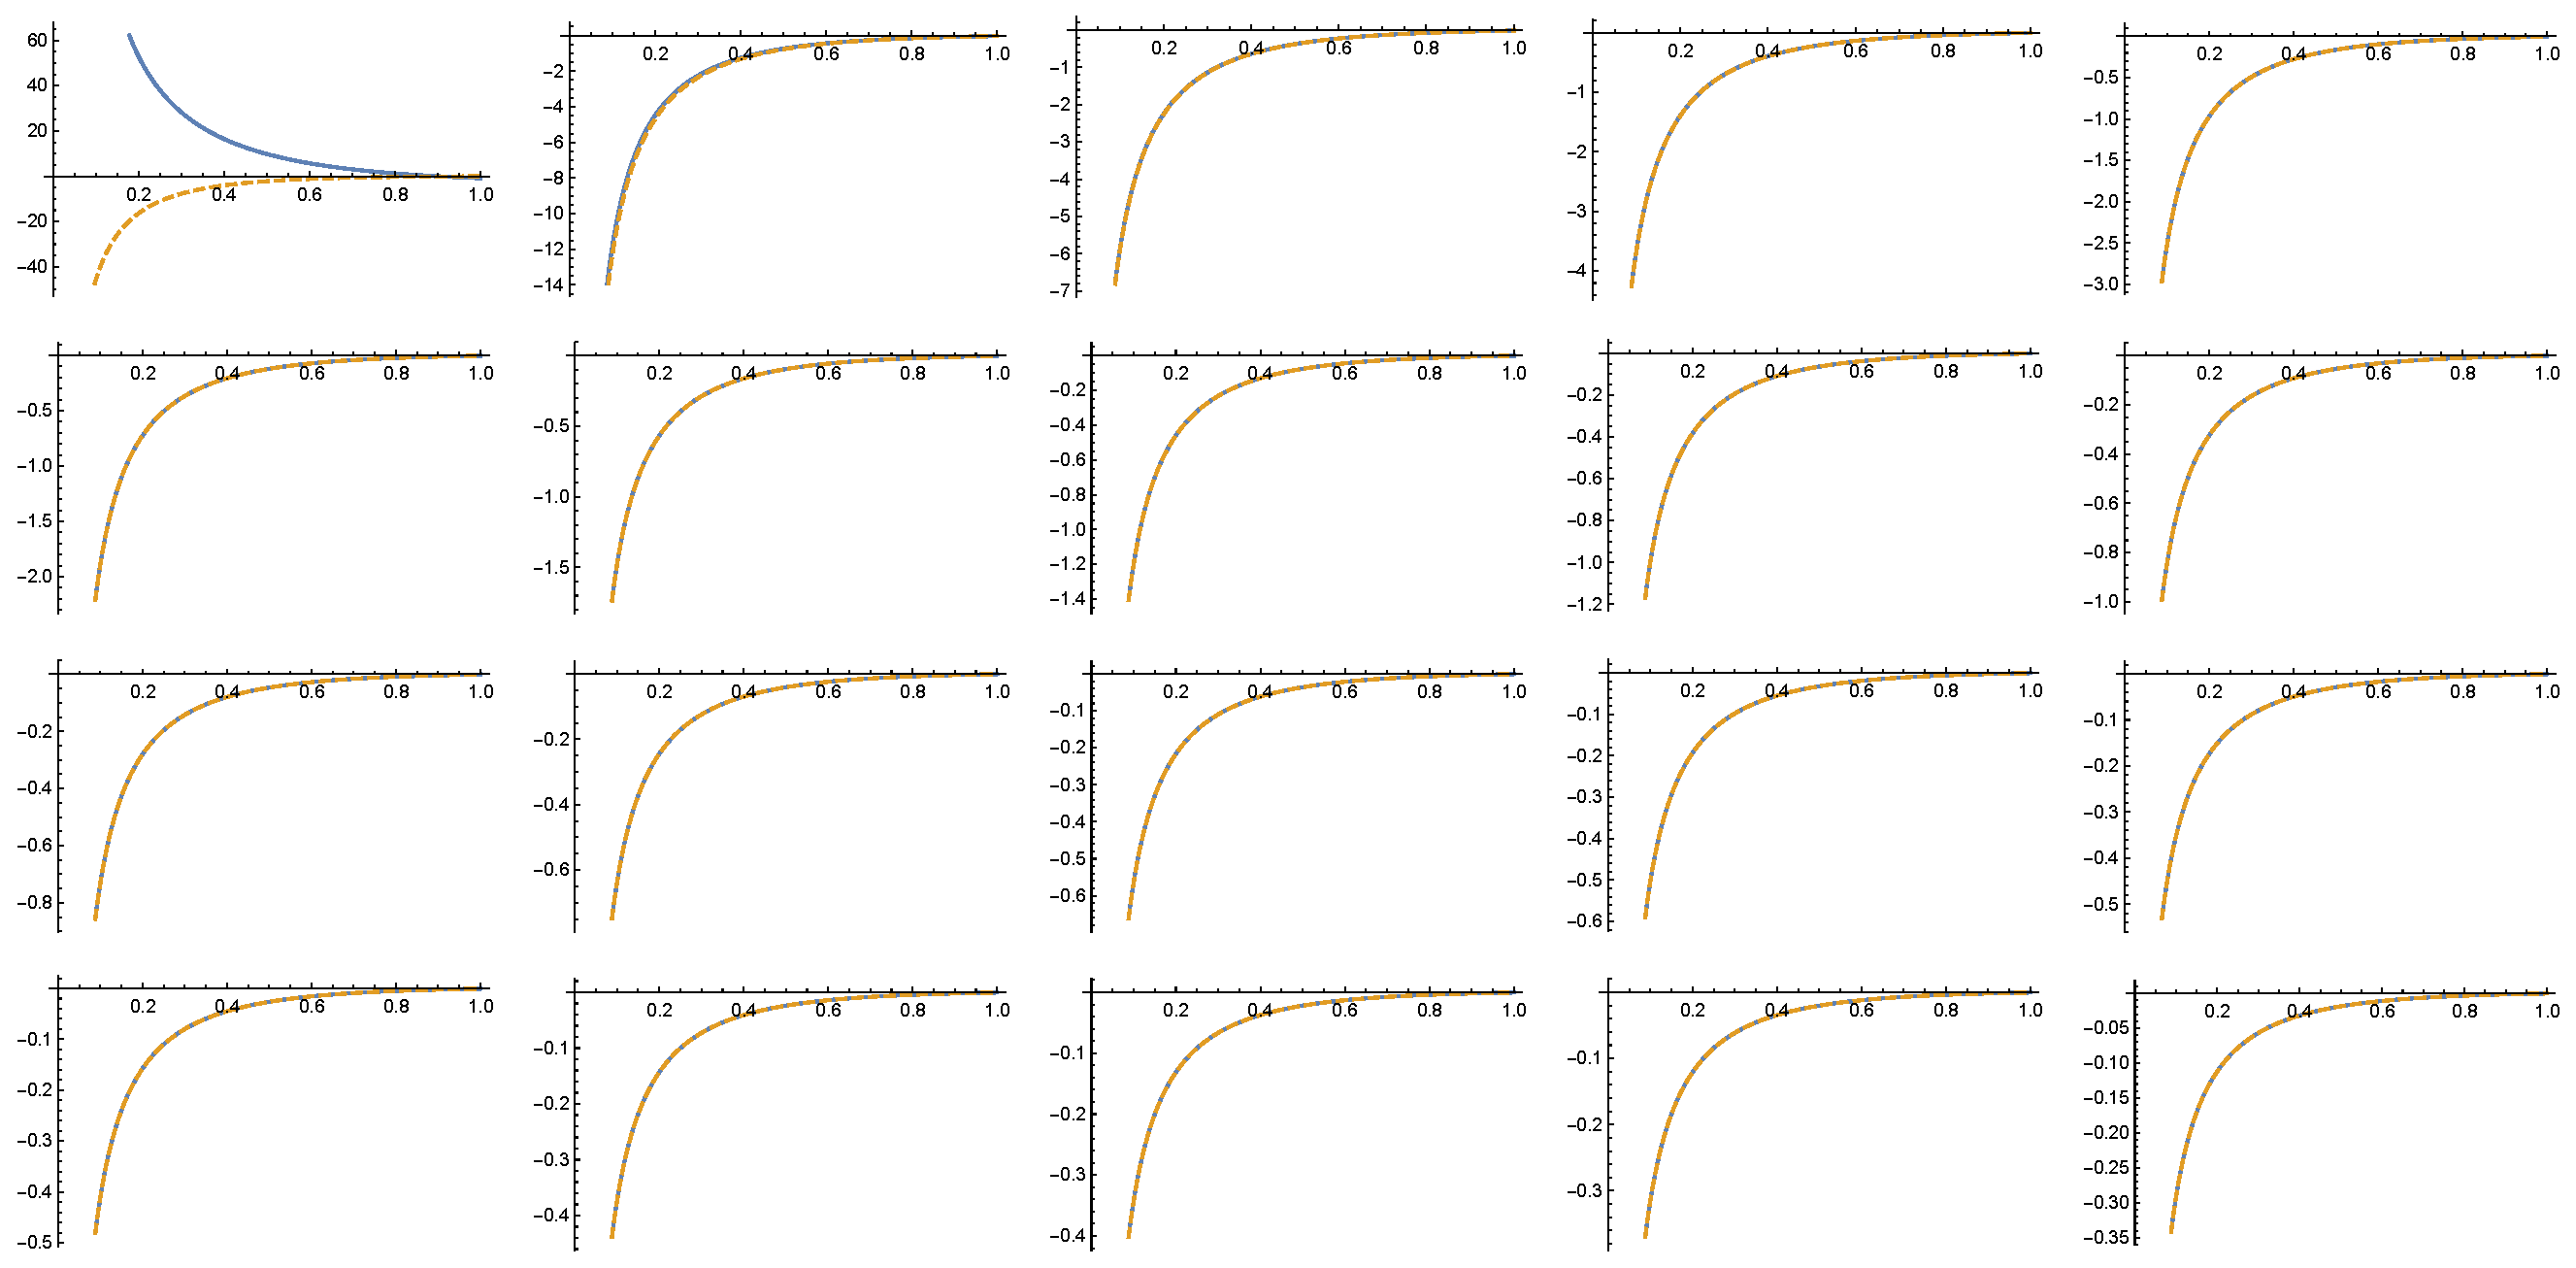
\includegraphics[width=6in]{psirlap.eps}
  \caption{$\psi_{eff}(r)(r<a)$在前20个能级与真实波函数的对比}
\end{figure}
\clearpage

\end{document}
